\documentclass{article}

% Input packages & formatting
% Packages

% Math packages
\usepackage{amsmath} % Extended math functions
\usepackage{amssymb} % Extended math symbols (loads in amsfonts)
\usepackage{bm} % Bold math symbols
\usepackage{mathtools}

% Figure packages
\usepackage{caption} % Caption formatting for university standard
\usepackage{graphicx} % includegraphics command
\usepackage{subcaption} % Subfigures
\usepackage[section]{placeins} % Place floats in section
\usepackage{wrapfig}

% Table packages
\usepackage{booktabs} % Better tables
\usepackage{bigstrut} % Merged table cells
\usepackage{longtable} % Tables which overflow into next page
\usepackage{array}
\usepackage{colortbl} % Color table cells
\usepackage{makecell}
\usepackage{multirow}

% Fonts
\usepackage{lmodern} % Use latin modern rather than computer modern. Better for font encoding.
\usepackage[T1]{fontenc} % Allow text to be searchable in output

% Other packages
\usepackage{appendix} % Appendix environment
\usepackage{nextpage} % Cleartooddpage command
%\usepackage[square,comma,sort,numbers]{natbib} % Reference formatting
\usepackage{setspace} % Line spacing
\usepackage{listings} % Display code with syntax highlighting
\usepackage{upquote} % Vertical quotes in verbatim
\usepackage{xcolor} % Colors
\usepackage{titlesec} % Header spacing
\usepackage{xparse} % for tcolorbox
\usepackage[listings]{tcolorbox} % Colored boxes for highlighting syntax
\tcbuselibrary{breakable}
\tcbuselibrary{skins}
\usepackage{enumitem} % better enumerate/itemize options
\usepackage{fancyhdr}
\usepackage{multicol}
\usepackage{ifthen}
\usepackage{xstring}

% Table of contents
\usepackage{imakeidx} % Index page
\usepackage{tocloft} % Control of table of contents
\usepackage[nottoc]{tocbibind} % Adds bibliography, table of tables, table of figures, to table of contents
\usepackage[bookmarks,linktocpage,hidelinks]{hyperref} % Hyperlinks for sections, figures, etc.

% Bibliography
\usepackage[style=numeric]{biblatex}
\addbibresource{references/references.bib}
% Formatting
% Page format
\setlength{\oddsidemargin}{0.00in}  % Left side margin for odd numbered pages
\setlength{\evensidemargin}{0.00in} % Right side margin for even numbered pages
\setlength{\topmargin}{0.00in}      % Top margin
\setlength{\headheight}{0.20in}     % Header height
\setlength{\headsep}{0.20in}        % Separation between header and main text
\setlength{\topskip}{0.00in}        % Top skip
\setlength{\textwidth}{6.50in}      % Width of the text
\setlength{\textheight}{8.50in}     % Height of the text
\setlength{\footskip}{0.50in}       % Foot skip
\setlength{\parindent}{0.00in}      % First line indentation
\setlength{\parskip}{6pt}        % Space between two paragraphs

% Captions (figures, tables, etc.)
\setlength{\floatsep}{\parskip}          % Space left between floats.
\setlength{\textfloatsep}{\floatsep}   % Space between last top float
% or first bottom float and the text
\setlength{\intextsep}{\floatsep}      % Space left on top and bottom
% of an in-text float
\setlength{\abovecaptionskip}{0.1in plus 0.25in}  % Space above caption
\setlength{\belowcaptionskip}{0.1in plus 0.25in}  % Space below caption
\setlength{\captionmargin}{0.50in}     % Left/Right margin for caption
\setlength{\abovedisplayskip}{0.00in plus 0.25in} % Space before Math stuff
\setlength{\belowdisplayskip}{0.00in plus 0.25in} % Space after Math stuff
\setlength{\arraycolsep}{0.10in}       % Gap between columns of an array
\setlength{\jot}{0.10in}                % Gap between multiline equations
\setlength{\itemsep}{0.10in}           % Space between successive items

% Counters (no section numbering)
\setcounter{tocdepth}{3}
\setcounter{secnumdepth}{0}

% Spacing
\setstretch{1.5}

\titlespacing*{\section}{0cm}{6pt}{6pt}[0cm]
\titlespacing*{\subsection}{0cm}{6pt}{6pt}[0cm]
\titlespacing*{\subsubsection}{0cm}{6pt}{6pt}[0cm]

\titleformat{\section}
{\sffamily\huge}{}{0pt}{\titlerule\vspace{-0.2cm}}
\titleformat{\subsection}
{\sffamily\itshape\Large}{}{0pt}{}

% Macro for syntax
\newtcolorbox{syntax}{
    size=small,
    sharp corners,
    colframe=black,
    colback=yellow,
    fontupper=\bfseries\ttfamily
}

% Macro for argument table
\newenvironment{args}{
    \begin{tabular}{>{\bfseries\ttfamily}p{0.25\linewidth} p{0.69\linewidth}}
    }{
    \end{tabular}\par
    \vspace{0.5\baselineskip}
}

% Note: Requires packages "listing", "xcolor", and "textcomp"
\lstdefinelanguage{verbatim}{
    basicstyle=\ttfamily\small,
    xleftmargin=9pt,
    xrightmargin=9pt,
    columns=fullflexible,
    keepspaces=true,
    comment=[l]{\#},
    breaklines=true
}

\lstdefinestyle{verbatim}{
    commentstyle=\color{gray},
}

% Example code
\AtBeginDocument{
\newtcolorbox[blend into=listings]{example}[2][]{
    colback=blue!3!white,
    colframe=black,
    colbacktitle=blue!15!white,
    coltitle=black,
    sharp corners,
    enhanced,
    breakable,
    size=small,
    before upper={
        \setstretch{1.0}\lstset{language=verbatim,style=verbatim}\vspace{3pt}\textsf{\textit{Code:}}
    },
    subtitle style={
        colback=blue!20!white,
        fonttitle=\sffamily
    },
    before lower={
        \setstretch{1.0}\lstset{language=verbatim,style=verbatim}\vspace{3pt}\textsf{\textit{Output:}}
    },
    fonttitle=\sffamily,
    title={#2},
    #1
}
}


% Links to sub and subsub commands - optional boolean argument, default true. if false, only displays subcmd.

% Commands (and command ensembles)
\newcommand{\command}[1]{\protect\hypertarget{#1}{#1}\index{#1}}
\newcommand{\subcommand}[2]{\protect\hypertarget{#1 #2}{#1 #2}\index{#1!#2}}
\newcommand{\cmdlink}[1]{\protect\hyperlink{#1}{\textit{#1}}}
\newcommand{\subcmdlink}[3][1]{\protect\hyperlink{#2 #3}{\ifnum#1=1\relax\textit{#2 #3}\else\textit{#3}\fi}}

% Methods (first arg is class)
\newcommand{\method}[2]{\protect\hypertarget{$#1Obj #2}{\$#1Obj #2}\index{#1!#2}}
\newcommand{\methodlink}[3][1]{\protect\hyperlink{$#2Obj #3}{\ifnum#1=1\relax\textit{\$#2Obj #3}\else\textit{#3}\fi}}

% Macros for figure/table names
\newcommand{\fig}{\figurename\ }
\newcommand{\figs}{\figurename s }
\newcommand{\tbl}{\tablename\ }
\newcommand{\tbls}{\tablename s }
\newcommand{\eq}{Eq. }
\newcommand{\eqs}{Eqs. }
\renewcommand{\lstlistingname}{Example}% Listing -> Example
\renewcommand{\lstlistlistingname}{List of \lstlistingname s}% List of Listings -> List of Examples
\newcommand{\ex}{Example }
\newcommand{\exs}{Examples }
\newcommand{\var}[1]{\texttt{\textbf{\$#1}}}

% Header/footer
\renewcommand{\headrulewidth}{0pt}

\fancypagestyle{main}{
\fancyhf{}
\fancyhead[RE,LO]{\textsf{Object-Oriented Incremental Dynamic Analysis (ooida)}}
\fancyhead[LE,RO]{\textsf{\thepage}}
}

\fancypagestyle{chapter}{
\fancyhf{}
\fancyfoot[LE,RO]{\textsf{\thepage}}
}

\fancypagestyle{foreword}{
\fancyhf{}
\fancyfoot[C]{\textsf{\thepage}}
}

% Changes to hyperlinks (URLs)
\renewcommand\UrlFont{\color{blue}\rmfamily}

% New column type 
% https://tex.stackexchange.com/questions/75717/how-can-i-mix-itemize-and-tabular-environments
\newcolumntype{L}{>{\labelitemi~~}l<{}}
\newcommand{\version}{0.2}

\newcommand{\caret}{$^\wedge$}

% Figure path and type
\pdfminorversion=6
\DeclareGraphicsExtensions{.pdf,.png}
\graphicspath{{./figures/}}

% Other macros
\renewcommand{\^}[1]{\textsuperscript{#1}}
\renewcommand{\_}[1]{\textsubscript{#1}}

\title{\LARGE Object-Oriented Incremental Dynamic Analysis (ooida)\\\small Version \version}
\author{Alex Baker\\\small\url{https://github.com/ambaker1/ooida}}
\date{\small\today}
\begin{document}
\maketitle
\clearpage
\section{General}
Incremental Dynamic Analysis (IDA) is a methodology for collapse assessment of buildings, and is essentially a parametric study, investigating the nonlinear response of a structure exposed to different earthquakes at increasing intensity. 
Of primary interest is to determine, at a high resolution, the collapse capacity of the structure for the given ground motion.
Of secondary interest is to trace the curve below the capacity point, to ensure that the capacity point is not part of a ``structural resurrection''.
The tracing algorithm used is based on the original ``hunt-fill'' algorithm by Vamvatsikos and Cornell  \cite{vamvatsikos_incremental_2002,vamvatsikos_performing_2011}, modified as described in \cite{baker_kinematics_2022}.

In similar fashion to the traditional hunt-fill tracing algorithm, the ``ooida'' package hunts for the capacity point and fills in the curve using a multi-staged approach:
\begin{enumerate}[label=\quad Stage \arabic*:,itemindent=*]
  \setcounter{enumi}{-1}
  \item Initialization stage, or simply the starting point. 
  \item ``Hunt-up'' stage, where it will increase the intensity until collapse is reached. 
  \item ``Bracketing'' stage, where it bisects to achieve desired precision on collapse capacity. 
  \item ``Fill-in'' stage, where the gaps below collapse are refined to achieve desired curve granularity. 
  \item Completion stage: collapse is reached and the all tolerances are met.
\end{enumerate}
\subsection{Installation and Use}
The ``ooida'' package and its dependencies can be installed with \textcolor{blue}{\href{https://github.com/ambaker1/Tin}{Tin}}, a package manager for Tcl.
The code below handles installation and importing of all commands.
\begin{example}{Installing and Importing ``ooida''}
\begin{lstlisting}
package require tin
tin add -auto ooida https://github.com/ambaker1/ooida install.tcl
tin import ooida
\end{lstlisting}
\end{example}


\clearpage
\section{Creating IDA Objects}
The command \cmdlink{ida} is a TclOO class based on the superclass \textit{::vutil::ValueContainer}, from the package \textcolor{blue}{\href{https://github.com/ambaker1/vutil}{vutil}}. 
It is an object-oriented approach to running Incremental Dynamic Analysis.
\begin{syntax}
\command{ida} new \$varName <\$value> <\$settings> \\
ida create \$name \$varName <\$value> <\$settings>
\end{syntax}
\begin{args}
\$varName & Variable to tie to IDA object. \\
\$value & Dictionary of intensity measures and collapse codes. Default blank. \\
\$settings & Settings dictionary. Default blank. See \methodlink{ida}{configure} for options.
\end{args}

\subsection{Copying IDA Objects}
The copy operator, ``\texttt{-{}->}'', copies the IDA to a new variable, and returns the new object.
\begin{syntax}
\index{ida methods!-{}->} \$idaObj -{}-> \$varName
\end{syntax} 
\begin{args}
\$varName & Variable to store object name for access and garbage collection. 
\end{args}

\subsection{Destroying IDA Objects}
Objects can either be destroyed with the method \methodlink[0]{ida}{destroy}, or by simply unsetting or overwriting the variable that it is tied to.
\begin{syntax}
\method{ida}{destroy}
\end{syntax} 

Below is a simple example of how you create, copy, and delete IDA objects
\begin{example}{Creating IDA objects}
\begin{lstlisting}
ida new x {1.0 0 2.0 1}; # create new IDA object
$x --> y; # copy IDA object to new variable
unset x; # destroys object stored in x
\end{lstlisting}
\end{example}
\clearpage

\subsection{Access/Modification}
The IDA data can be accessed by calling the IDA object without any methods, and the value can be overwritten with the assignment operator ``\texttt{=}''. 
The assignment operator returns the IDA object.
\begin{syntax}
\index{ida methods!=} \$idaObj = \$value
\end{syntax}
\begin{args}
\$value & Dictionary of intensity measures and collapse codes.
\end{args}

The methods \methodlink[0]{ida}{set} and \methodlink[0]{ida}{unset} add or remove points from the IDA curve.
Both methods return the object.

\begin{syntax}
\method{ida}{set} \$im \$code
\end{syntax}
\begin{args}
\$im & Intensity measure. \\
\$code & Boolean collapse code. 0 for no collapse. 
\end{args}

\begin{syntax}
\method{ida}{unset} \$im
\end{syntax}
\begin{args}
\$im & Intensity measure. 
\end{args}

\begin{example}{Creating and Modifying IDA objects}
\begin{lstlisting}
ida new x; # create new IDA object
$x = {1.0 0 2.0 1}
$x set 1.5 1
$x unset 2.0
puts [$x]
\end{lstlisting}
\tcblower
\begin{lstlisting}
1.0 0 1.5 1
\end{lstlisting}
\end{example}
\clearpage

\section{IDA Configuration}
The settings of an IDA object can be queried and modified with the method \methodlink[0]{ida}{configure}.
If this method is called with no arguments, it returns a dictionary of all configuration settings. 
If called with a single argument, it will return the current configuration for the specified setting. 
If called with more than one argument, the input will be parsed as a paired list of settings and configuration values to apply, and it will return the object.
\begin{syntax}
\method{ida}{configure} \\
\$idaObj configure \$option \\
\$idaObj configure \$option \$value ...
\end{syntax}
\begin{args}
\$option ... & Setting options to set or query. \\
\$value ... & Configuration values for settings.
\end{args}
\FloatBarrier
\subsection{Initialization}
The initial intensity measure used for a blank IDA can be configured with the \textit{-start} configuration setting.
If not specified, it will default to ``1.0''.
\begin{syntax}
\$idaObj configure -start \$init
\end{syntax}
\begin{args}
\$init & Starting intensity measure. Default 1.0. \\
\end{args}
\clearpage
\subsection{Hunt-up Method}
The algorithm used to determine the next intensity measure prior to collapse is defined with the \textit{-huntup} configuration setting.
If not specified, it will default to ``Geometric 2.0''.
\begin{syntax}
\$idaObj configure -huntup "\$type \$step"
\end{syntax}
\begin{args}
\$type & Hunt-up method (\textit{Geometric}, \textit{Quadratic}, or \textit{Linear}. Default \textit{Geometric}) \\
\$step & For \textit{Geometric}, the geometric ratio. For \textit{Quadratic}, the step increase. For \textit{Linear}, the step size. Default 2.0.
\end{args}
The \textit{Geometric} method ensures that the ratio between gaps is constant, while the \textit{Quadratic} method ensures that the difference between gaps is constant. To illustrate their differences, the hunt-up of a simple IDA curve $(\text{DM} = \text{IM}^2)$ is performed with both methods with the same number of steps and the same start and end point, as shown in \fig\ref{fig:ida_huntup}.

As can be seen in the figure, the \textit{Geometric} method can increase gap size more quickly, while the \textit{Quadratic} method produces more consistent gap sizes. 
\begin{figure}[!htb]
\centering
\begin{subfigure}[b]{0.45\linewidth}
    \centering
    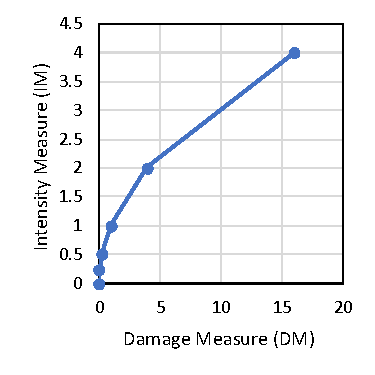
\includegraphics[width=2.5in]{ida_geometric_huntup}
    \caption{Geometric Hunt-up: \newline Start = 0.25, Step = 2.0}
    \label{fig:ida_geometric_huntup}
\end{subfigure}
\begin{subfigure}[b]{0.45\linewidth}
    \centering
    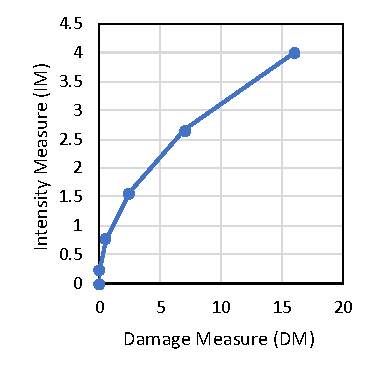
\includegraphics[width=2.5in]{ida_quadratic_huntup}
    \caption{Quadratic Hunt-up: \newline Start = 0.25, Step = 0.275}
    \label{fig:ida_quadratic_huntup}
\end{subfigure}
\caption{Geometric vs Quadratic Hunt-up}
\label{fig:ida_huntup}
\end{figure}
\clearpage
\subsection{Tolerances for Bracketing and Fill-In}
The tolerances for the Bracketing and Fill-In stages of the algorithm are defined with the \textit{-precision} configuration setting. If not specified, it will default to ``0.25 0.5''.
\begin{syntax}
\$idaObj configure -precision "\$eps1 \$eps2"
\end{syntax}
\begin{args}
\$eps1 & Bracketing stage tolerance. Default 0.25 \\
\$eps2 & Fill-in stage tolerance. Default 0.5
\end{args}
Once collapse is reached in the IDA algorithm, the algorithm will focus first on meeting tolerance on the collapse point. 
This is the Bracketing stage, where the gap between the capacity bounds is bisected until the gap is less than the tolerance.
When the bracketing tolerance is met, the algorithm enters the Fill-In stage, which focuses on meeting tolerance between points below the collapse point.
For the Fill-In stage, the gaps below the collapse point are bisected or trisected, going in order of largest gaps first, until no gap exists that is greater than the specified tolerance.
When both precision tolerances are met, the IDA curve is considered to be complete. 
\\

\begin{figure}[!htb]
\centering
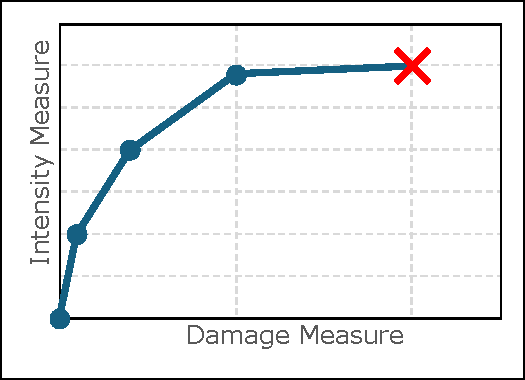
\includegraphics{ida_curve}
\caption{Representative IDA Curve}
\label{fig:ida_curve}
\end{figure}


\clearpage
\subsection{IDA Curve Refining Limits}
The lower and upper limits for refining the IDA collapse point are defined with the \textit{-limits} configuration setting.
This can be used to do partial IDAs as described in the FEMA P-695 methodology \cite{fema_quantification_2009}.
If not specified, it will default to ``0.0 Inf''.
\begin{syntax}
-limits "\$min \$max"
\end{syntax}
\begin{args}
\$min & Lower limit for refining collapse point. \\
\$max & Upper limit for refining collapse point.
\end{args}

The limits define three intensity measure zones as shown in \fig\ref{fig:ida_zones}. 
In the figure, if collapse has not been reached, the minimum collapse can be considered to be in zone 3. \\

\begin{figure}[!htb]
\centering
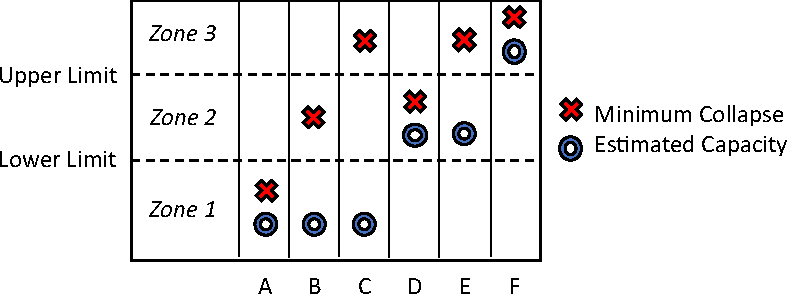
\includegraphics{ida_zones}
\caption{Partial IDA Zones}
\label{fig:ida_zones}
\end{figure}



Depending on which zones the the capacity and minimum collapse points are, it will modify the behavior of the IDA as described below:

\begin{tabular}{cp{0.9\linewidth}}
A & Both estimated capacity and minimum collapse are in zone 1. No more runs are required. \\
B & Capacity is below lower limit, but minimum collapse is above. Fill-in stage is not needed. \\
C & Same as B.\\
D & Both estimated capacity and minimum collapse are in zone 2. Full refinement is necessary to capture any structural resurrections. \\
E & Same as D. \\
F & Both estimated capacity and minimum collapse are in zone 3. Hunting and bracketing are not required, but curve must be filled in below upper limit to capture any structural resurrections.
\end{tabular}
\clearpage
\section{IDA Results}
The IDA dictionary and the configuration settings are used to analyze and determine the stage of the analysis, the next intensity measure to run, and what the estimated bounds are on collapse capacity.

The stage of the IDA can be queried with the method \methodlink[0]{ida}{stage}.
\begin{syntax}
\method{ida}{stage}
\end{syntax}

The next intensity measure can be queried with \methodlink{ida}{next}. 
If the IDA is complete, it will return blank.
\begin{syntax}
\method{ida}{next}
\end{syntax}

The lower and upper limits on collapse capacity can be queried with the method \methodlink[0]{ida}{capacity}.
The upper limit is the minimum collapse if collapse is reached.
\begin{syntax}
\method{ida}{capacity}
\end{syntax}

Below is an example of how to use the IDA framework to run an analysis.
\begin{example}{Example Application}
\begin{lstlisting}
# Define place-holder collapse equation (with structural resurrection)
proc Collapsed {x} {
    expr {$x >= 7.5 || ($x > 3.0 && $x <= 3.5)}
}
# Create IDA object
ida new ida {} {
    -huntup {Geometric 2.0}
    -precision {0.25 0.5}
}
# Run IDA
while {[$ida stage] < 4} {
    set im [$ida next]
    $ida set $im [Collapsed $im]
}
# Print out capacity, and history of analysis
puts [$ida capacity]
puts [dict keys [$ida]]
\end{lstlisting}
\tcblower
\begin{lstlisting}
3.0 3.25
1.0 2.0 4.0 8.0 6.0 7.0 7.5 7.25 3.0 5.0 0.5 1.5 2.5 3.5 3.25
\end{lstlisting}
\end{example}


\phantomsection
\interlinepenalty=1000
\printbibliography[heading=bibintoc]
\end{document}
